\documentclass[10pt,a4paper]{article}
\usepackage[utf8]{inputenc} % para poder usar tildes en archivos UTF-8
\usepackage[spanish, es-tabla]{babel} % para que comandos como \today den el resultado en castellano
\usepackage{a4wide} % márgenes un poco más anchos que lo usual
\usepackage[conEntregas]{caratula}
\usepackage{xcolor,colortbl}
\usepackage{todonotes}
\usepackage{graphicx}
\usepackage{subcaption}
\usepackage{algorithm}
\usepackage{algorithmic}
\usepackage{cite}

%definations
\definecolor{Gray}{gray}{0.6}
\definecolor{ligthGray}{gray}{0.9}
\newcommand{\mc}[2]{\multicolumn{#1}{|c|}{#2}}

\begin{document}

\titulo{NetworkDEVS}
\subtitulo{Una herramienta de estudio para medelar redes usando DEVS y PowerDEVS}

\fecha{\today}

\materia{Teoría de las telecomunicaciones}

\integrante{Belloli, Laouen Mayal Louan}{134/11}{laouen.belloli@gmail.com}

\maketitle

\tableofcontents
\newpage

\section{Introducción y Motivación}

El presente trabajo se introduce un modelo DEVS de una red funcionando bajo el protocolo TCP/IP encuadrando lo mejor posible cada uno de sus módulos en su correspondiente capa respecto al modelo OSI presentado en la literatura oficial de la materia de teoría de la telecomunicaciones \cite{peterson2007computer}. El trabajo fue desarrollado en el simulador PowerDEVS y pensado como herramienta de aprendizaje para futuros alumnos de la materia.

El principal aporte de este trabajo consiste en la creación de un framework que permite programar y modificar los protocolos de una red de telecomunicaciones para luego simular su comportamiento y obtener feedback instantáneo de los resultados. Además, usando el simulador PowerDEVS, se consigue brindar una interfaz gráfica intuitiva que mapea de forma directa los dispositivos de la red con los módulos del modelo. Esta interfaz gráfica permite también crear distintos escenarios topológicos sin tener que tocar ni una linea de código. 

Por otro lado, esta interfaz gráfica permite modularizar de forma explicita las distintas capas del modelo y su interacción, mapeando los modelos DEVS de cada capa con su capa correspondiente en la red, permitiendo una interacción más tangible y concreta respecto al modelo en capa. De esta forma, se programa cada protocolo en su capa correspondiente, esto no es menor, ya que si bien, teóricamente, los distintos protocolos están separados en capas y las redes pueden ser pensadas en capas, en la realidad, estas capas no existen de forma explicita y hay un salto entre las teorías de redes y los modelos en capas respecto de sus distintas implementaciones prácticas donde las capas terminan mezclándose en varios aspectos. Este modelo, permite a los alumnos hacer trabajos prácticos donde implementar los protocolos manteniendo explicitas las capas y por ende, acercando la teoría y la práctica de las redes de telecomunicaciones.

Si bien, el modelo realizado es un modelo DEVS (Discrete EVent System Specification), el mismo fue pensado para que no sea necesario más que una breve introducción a DEVS, por lo que mismo personas sin ninguna experiencia en DEVS deberían ser capases de poder utilizar el simulador, el modelo y el framework general propuesto en este trabajo.

\section{Objetivos}

Los objetivos de este trabajo se pueden dividir en varias partes:
\subsection{Introducir un framework para modelos de redes}

Como ya fue mencionado en la introducción, uno de los principales objetivos de este trabajo es implementar un framework, que permita fácilmente implementar protocolos de red y validarlos mediante Simulación de Eventos Discretos (DES) generando distintos escenarios. Esto permite testear los protocolos implementados de forma sencilla y rápida. Obteniendo una herramienta útil, tanto para el estudio de las redes de telecomunicaciones como para la investigación en el área. 

La creación de un modelo que sirva como framework, tiene por objetivo factorizar y estandarizar las partes comunes a todos los protocolos, estás partes comunes provienen de las propiedades inherentes a los dispositivos físicos en los cuales los protocolos están corriendo, y de los estándares actualmente utilizados que permiten obtener robustez y compatibilidad entre distintas implementaciones que puedan existir en distintas partes de una red. Estas abstracciones encapsuladas en el modelo framework presentado, permiten al modelador, concentrarse plenamente en su protocolo y permite la reutilización y compatibilidad de distintos modelos que pueden luego ser combinados en un único modelo de una red que funcione bajo distintos protocolos, permitiendo así el estudio de la compatibilidad y homogeneidad de los protocolos implementados.

\subsection{Implementar un modelo UDP/IP básico}

Por otro lado, este trabajo pretende implementar un modelo básico de una red UDP/IP que permita cubrir los protocolos mínimos e indispensables para hacer funcionar una pequeña red. Este modelo no tiene como intensión implementar todas las partes, ni cubrir todos los protocolos de forma completa, por lo que temáticas como la fragmentación de paquetes, congestión de tráfico, el manejo de errores, Dinamic Host Configuration Protocol (DHCP) \cite[p.~231]{peterson2007computer}, Routing Information Protocol (RIP)\cite[p.~243]{peterson2007computer} y Spanning tree protocol \cite[p.~194]{peterson2007computer} quedan fuera del alcance de este trabajo, siendo los mismos posibles trabajos futuros.

También se implementó un modelo de switch que utiliza el protocolo de Datagramas \cite{petersonSwitchDatagram} utilizando una forwarding table para enviar los Frames por la interface correspondiente. 

\subsection{Mapeo entre el modelo UDP/IP y el modelo OSI}

En este trabajo, también pretendemos mostrar como se pueden implementar los distintos protocolos del modelo UDP/IP encuadrandolos en un modelo en capas OSI. Para esto, varias decisiones tuvieron que tomarse, siendo tal vez la más difícil, decidir en que capa implementar el protocolo ARP \cite[p.~228]{peterson2007computer}. Para tomar estas decisiones, se tomaron siempre como referencia los textos del libro \cite{peterson2007computer}. Se intentó también separar lo mejor posible las tareas de cada capa de forma tal que cada una de ellas pueda ignorar lo más posible la existencia de la/las capa/s inferior/es.

\section{Introdución a DEVS}
\section{Introducción a PowerDEVS}
\section{Arquitectura general}

La arquitectura general del modelo propuesto en este trabajo tiene por principal objetivo ofreser un framework donde se pueda facilmente desarrollar protocolos, para esto, se concentra en resolver varios puntos principales:

\begin{itemize}
\item Estandarizar la comunicación entre las capas de forma de conseguir consenso entre los distintos modeladores que usen esta herramienta, y que facilite una comprensión herarquica y organizada del modelo entero para los lectores nuevos.
\item Implementar todas aquellas partes generales a todos los modelos de protocolos de forma que solo sea necesario consentrarse en el protocolo a implementar.
\item intentar minimizar lo más posible la necesidad de tener conocimientos avanzados sobre DEVS a la hora de utilizar la herramienta.
\end{itemize}

La arquitectura consiste en un modelo de $N$ capas, con $N > 0$ de forma que cada capa $i, i \in [2,..,N-1]$ se comunica con las capas $i+1$ e $i-1$ utilizando $8$ canales de comunicación distintos:

\begin{itemize}
\item Output port 0: Envio de datos a la capa $i+1$.
\item Output port 1: Envio de controles a la capa $i+1$.
\item Output port 2: Envio de datos a la capa $i-1$.
\item Output port 3: Envio de controles a la capa $i-1$.
\item Input port 0: Recepción de datos de la capa $i+1$.
\item Input port 1: Recepción de controles de la capa $i+1$.
\item Input port 2: Recepción de datos de la capa $i-1$.
\item Input port 3: Recepción de controles de la capa $i-1$.
\end{itemize}

Dado que no siempre sucede que en un dispositivo de la red, exista un solo modulo por capa, por ejemplo, puede pasar que un host tenga varias aplicaciones enviando datos a travez de distintos sockets y en ese escenario habria más de un módulo en la capa de aplicación (capa siete del modelo OSI) de ese host, o un router probablemente tenga más de una interfaz, ya que suele tener una interfaz por cada sub-red a la cual esté conectado, entonces tendría más de un modulo en la capa de linkeo (capa dos del modelo OSI), y dado que los puertos de salida y entradas estan pensados para comunicarse con un solo modelo en la capa superior/inferior. Es necesario usar modelos demultiplexers que permitan redirigir los mensajes salientes por un puerto al modelo correspondiente de entre todas las posibles opciones. También, es necesario usar modelos multiplexers para que los múltiples modelos de la capa superior e inferior puedan enviarle mensajes al modulo. Esto se explicará más adelante con mayor detalle.

Las capas $1$ y $N$ usan la misma arquitectura que el resto de las capas y tienen definidos los mismos puertos. Dado que en la realidad existe solo un medio de comunicación entre dispositivos y tanto datos como controles se envian por ese medio, entonces el modelo acoplado "dispositivo" tiene solo un puerto de salida y un puerto de entrada destinado a enviar datos de cualquier tipo (datos o controles), y queda en el modelador decidir que puerto o puertos de salida de la capa $1$ conectar con el puerto de salida del modelo acoplado "dispositivo" y que puerto o puertos de entrada de la capa $1$ comunicar con los el puerto de entrada para datos. Por otro lado, el input necesario para la capa $N$ (comunmente el input que indica los comandos del usuario de enviar o recibir datos) se puede conectar directamente con los puertos de entrada de la capa $N$, ya sea dejando los modelos de input adentro de l modelo acoplado del "dispositivo" o afuera del mismo. Lo mismo ocurre con el output generado por la capa $N$ para las capas superiores que no existen, este output puede ser recibido por modelos que lo guardan en archivos, estos modelos también pueden estar definidos tanto adentro como afuera del modelo acoplado "dispositivo".\todo[linecolor=red,backgroundcolor=red!25,bordercolor=red]{Revisar esto}


Distintos dispositivos de la red pueden tener distintas cantidades de capas, por lo cual, la cantidad de capas existente puede variar entre los distintos modelos de cada dispositivo dentro de una misma red. Los host por ejemplo, suelen tener hasta la capa siete mientras que los routers comunes llegan a la capa tres y los switches a la capa dos.

La figura \ref{figure:general architecture} muestra la arquitectura general recien explicada en un modelo de una red con un host y un router, en el mismo se pueden se pueden ver los multiplexers y demultiplexers, se puede ver que cada modelo tiene distintas cantidadesde capas y se puede ver como estan conectadas las capas utilizando los distintos puertos.

\begin{figure}[htbp]
    \centering
    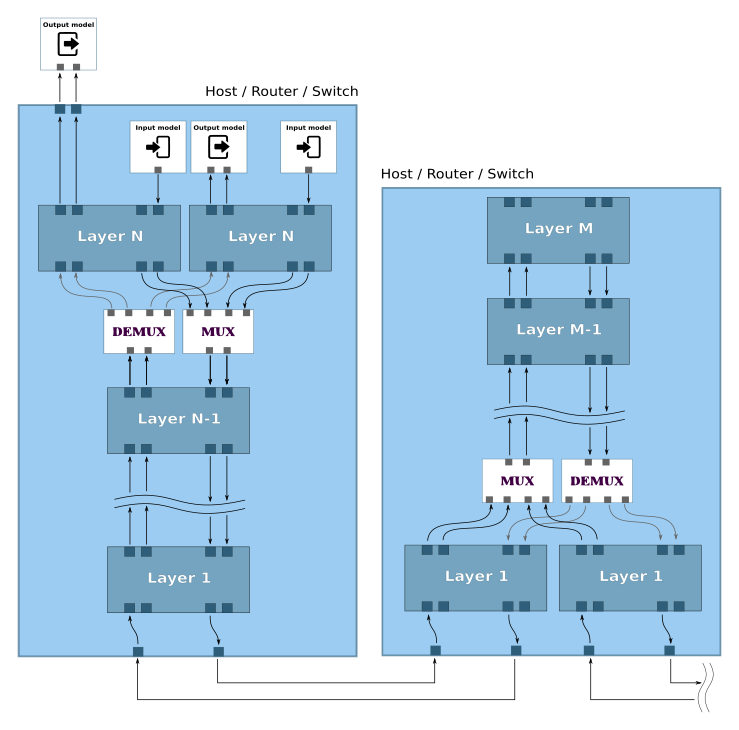
\includegraphics[width = 0.8\textwidth]{png/multi_layer_model.png}
    \caption{Arquitectura de un modelo en NetworkDEVS con dos dispositivos (un host y un reouter de N y M capas correspondientemente).}
    \label{figure:general architecture}
\end{figure}

\section{Como usar el template}
\subsection{Como heredar el modelo layer}
\subsection{Como enviar y recibir mensajes entre las capas}
\subsection{Como implementar el protocolo de una capa (internal/external functions)}
\section{Como agregar una capa}
\section{Como modificar un protocolo}
\section{Input/output del modelo}
\section{Logger}
\section{Case study: escenario implementado}
\section{Protocolos implementados}
\subsection{UDP}
\subsection{IP}
\subsection{ARP}
\subsection{SWP}
\subsection{Datagram protocol}
\section{Resultados}
\section{Conclusiones}
\section{Trabajo futuro}
\section{References}
\bibliographystyle{plain}
\bibliography{references}

\end{document}